
\chapter{TP2 : Outil de simulation de réseaux : NS-2}

    \section{Exercice 1: Protocoles de Routage}
    \subsection{Etablissement du réseau}
      On commence par réaliser le réseau demandé. Grâce au TP précédent, cela se fait rapidement, et selon les spécifications du sujet. On organise le code de la même façon que dans le TP précédent, pour plus de clareté. Le but de ce TP est de comparer les différences en termes de convergence, mise à jour de routage, et du comportement autour du noeud n5 de deux protocoles de routage, à Vecteur de distance et à Etat de lien. En ne changeant que ce facteur lors de 2 simulations, on pourra, à l'aide des outils fournis dans nam, facilement distinguer ce qui advient des paquets en transit pendant la perte de connexion, et comment les différents noeuds du réseau communiquent afin de réaliser le routage.
    \subsection{Vecteur Distance}
      Lors de la rupture, les paquets sont perdus, et le reroutage se met en route au bout de 30 ms. Lorsque la jonction est rétablie, le routage initial, plus court (dans les termes choisis par ns2) reprend lieu au bout de 10ms. Le protocole à Vecteur de Distance nécessite l'envoi de paquets périodiques (2s dans ns2) afin de maintenir le routage à jour, mais aussi lors du changement d'une distance au sein du réseau. Il s'agit donc d'une convergence lente.
    \subsection{Etat de liens}
      Lors de la rupture, cette fois-ci, les paquets ne sont pas perdus, ils sont simplement reroutés dès que possible, c'est-à-dire, quand une route est trouvée, au bout de 10ms (plus rapide qu'avec le protocole DV). Lorsque la jonction est rétablie, le routage reprend sa forme initiale, puisque plus rapide, et les paquets transitent comme avant la rupture au bout de 10ms. Ce protocole ne nécessite pas l'envoi de paquets périodiques, et pèse donc moins sur la congestion du réseau, par contre il nécessite l'envoi de paquets à chaque changements d'état d'une jonction. Étant plus rapide que le porotocole DV, on peut dire qu'il s'agit ici d'une convergence rapide.
    \section{Exercice 2: Routage et contrôle de congestion TCP}
      On réalise le réseau demandé, selon les spécifications précisées. On trace la courbe d'évolution de la fenêtre TCP (figure 1) en fonction du RTT, on précise la valeur de ssthresh et rwnd, et on détaille le nom des phases de l'évolution.

      Contrairement à l'exercice 2 du TP1, où il y avait de la congestion dû à trop de demandes d'utilisation du réseau, ici, une liaison est coupée. Il pourrait aussi y avoir des collision si le réseau était organisé différemment, causant la perte de paquets TCP.
      \vskip1ex
    \begin{figure}
    \centering
    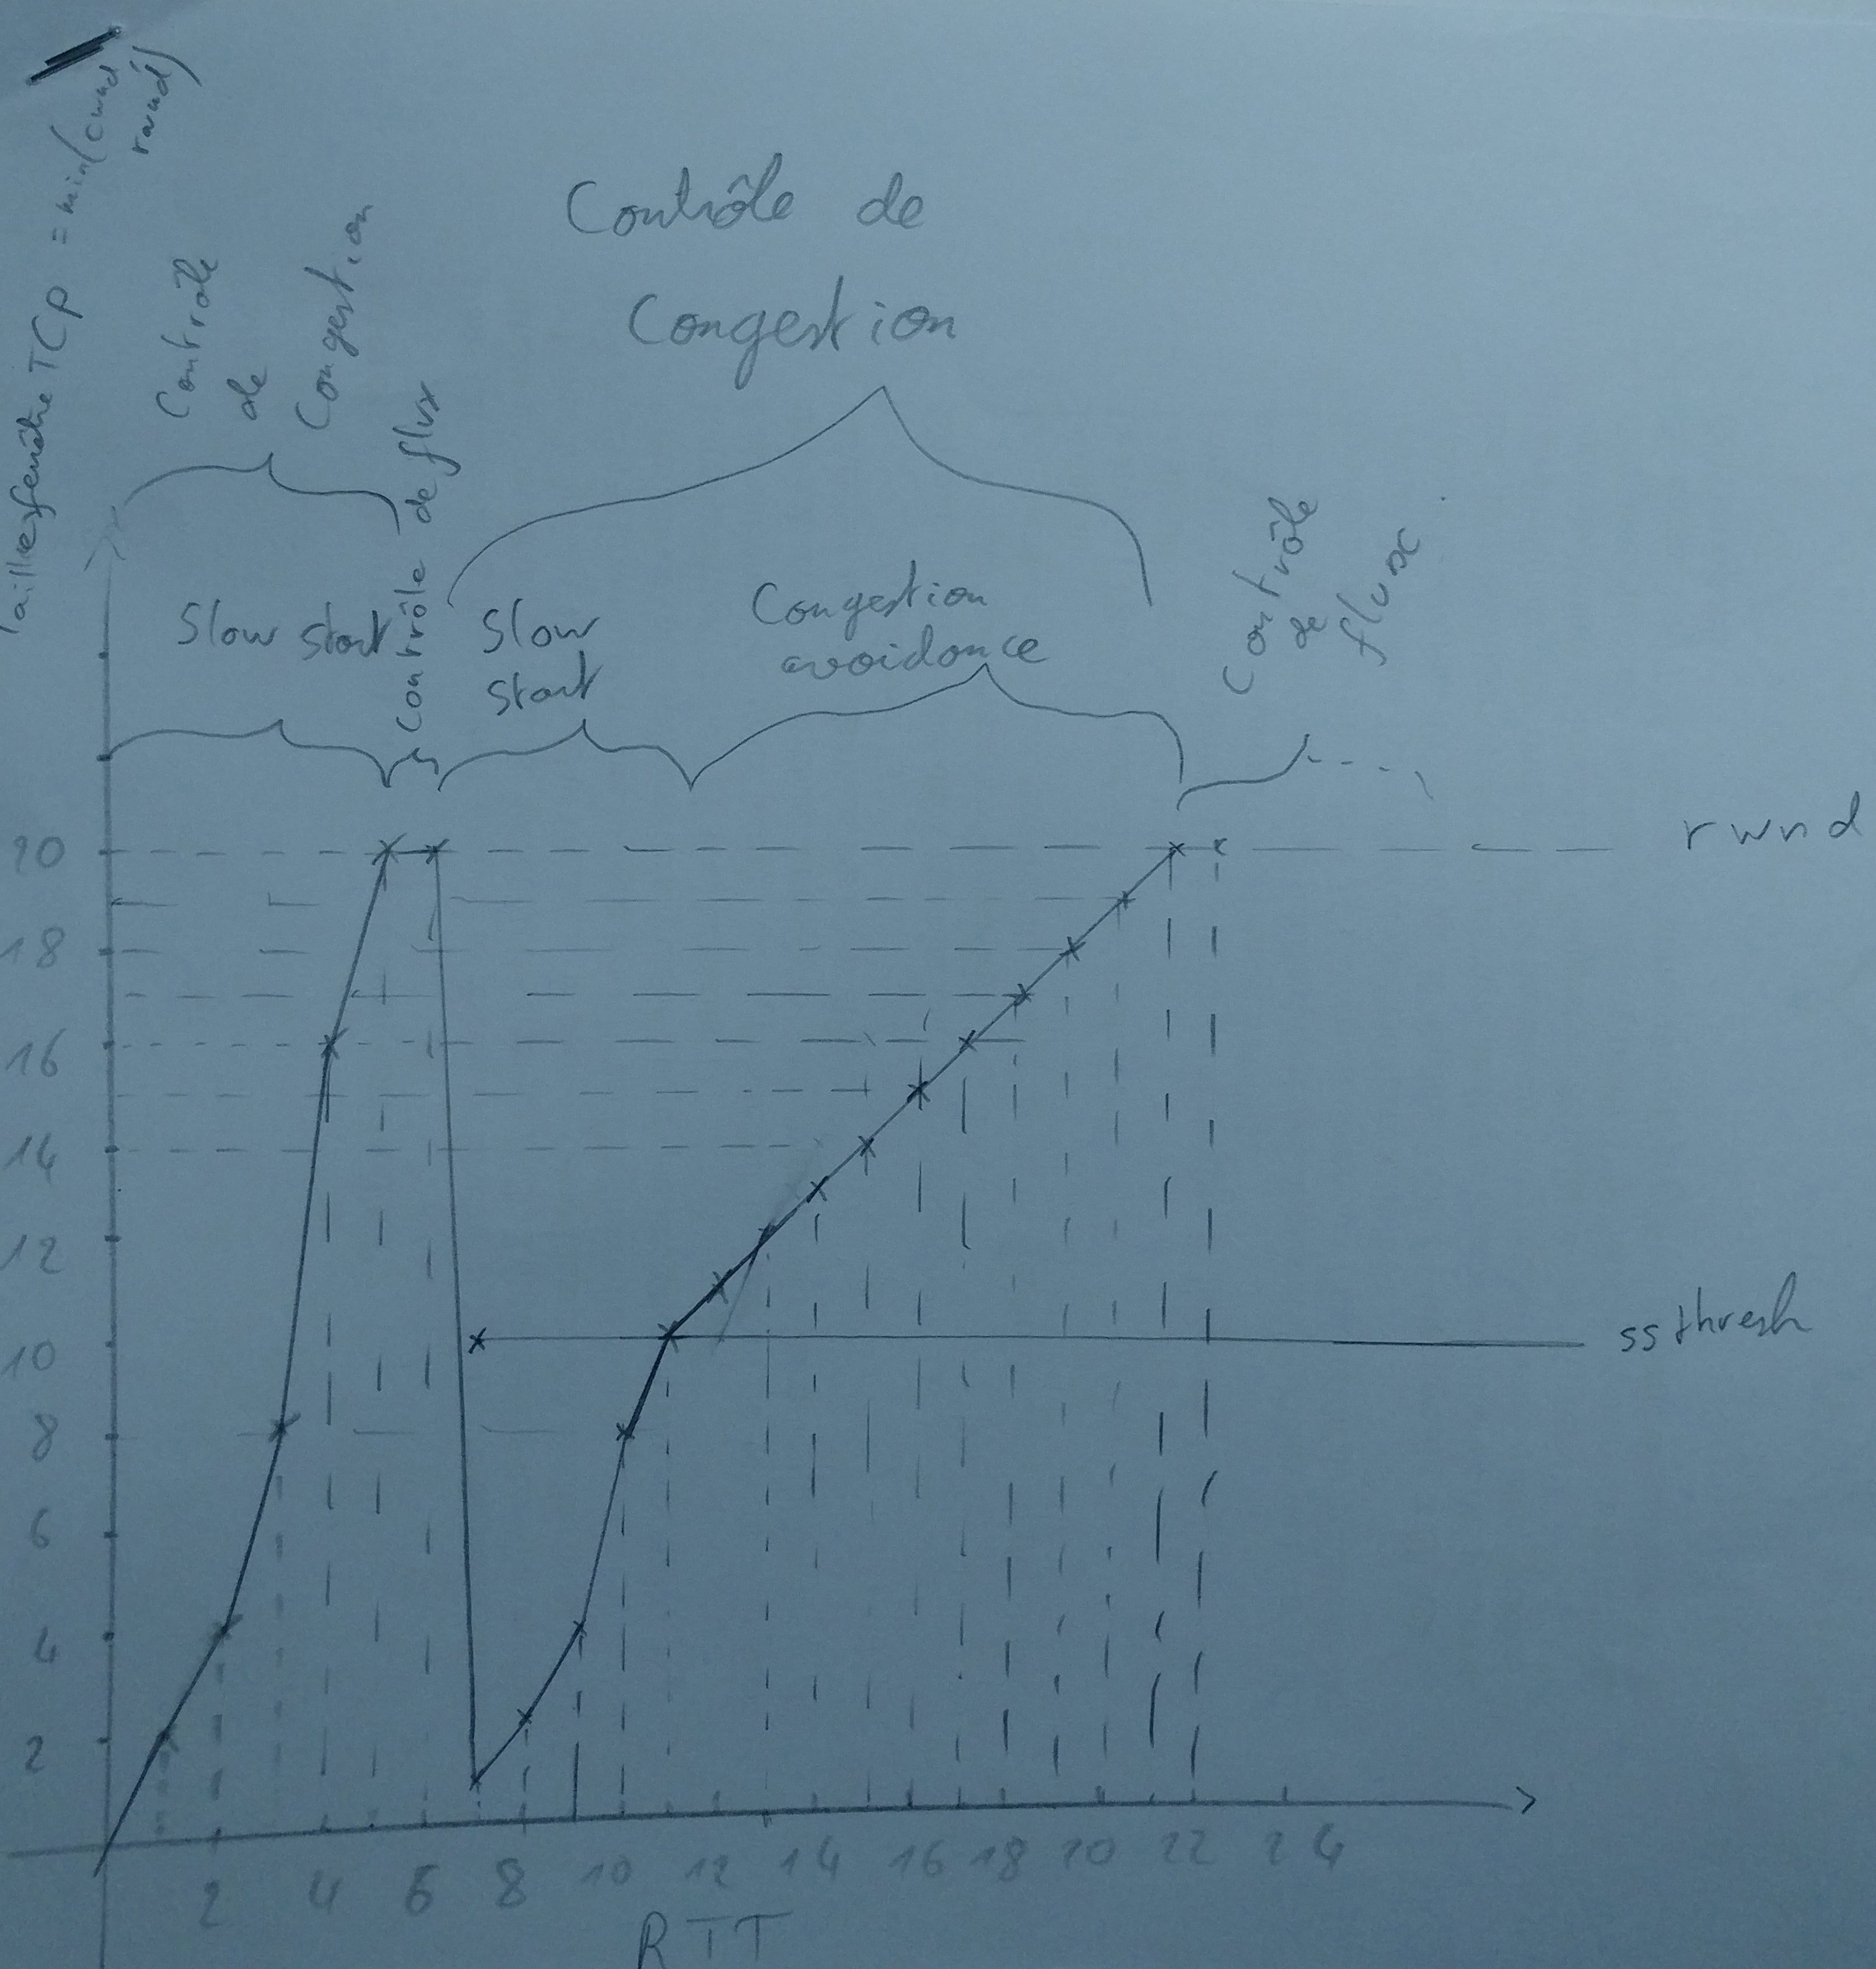
\includegraphics[width=0.99\columnwidth]{./tp2/courbe.jpg}
    \caption{Courbe d'évolution de la fenêtre TCP en fonction du RTT}
    \end{figure}
    \vskip1ex
    \begin{figure}
    \centering
    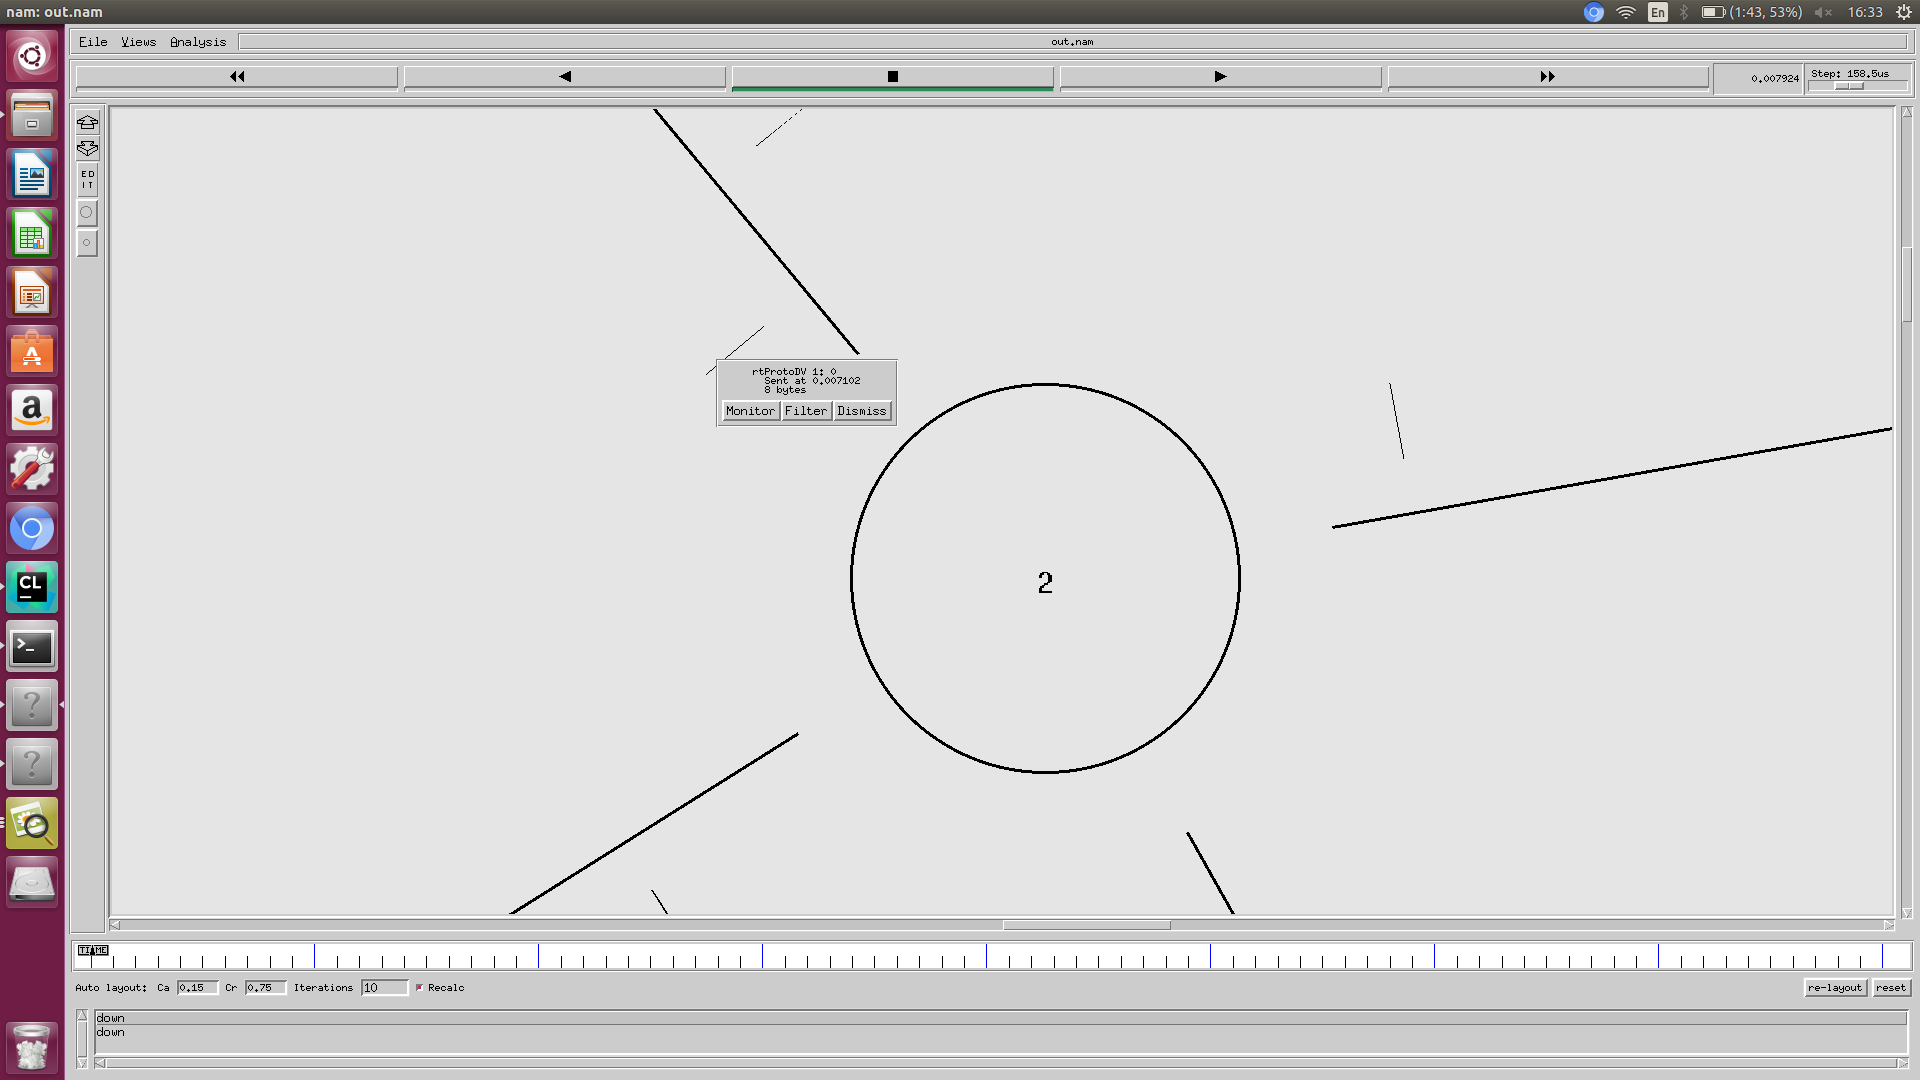
\includegraphics[width=0.99\columnwidth]{./tp2/tp2-1-DV-1-init.png}
    \caption{Initialisation du routage}
    \end{figure}
    \vskip1ex
    \begin{figure}
    \centering
    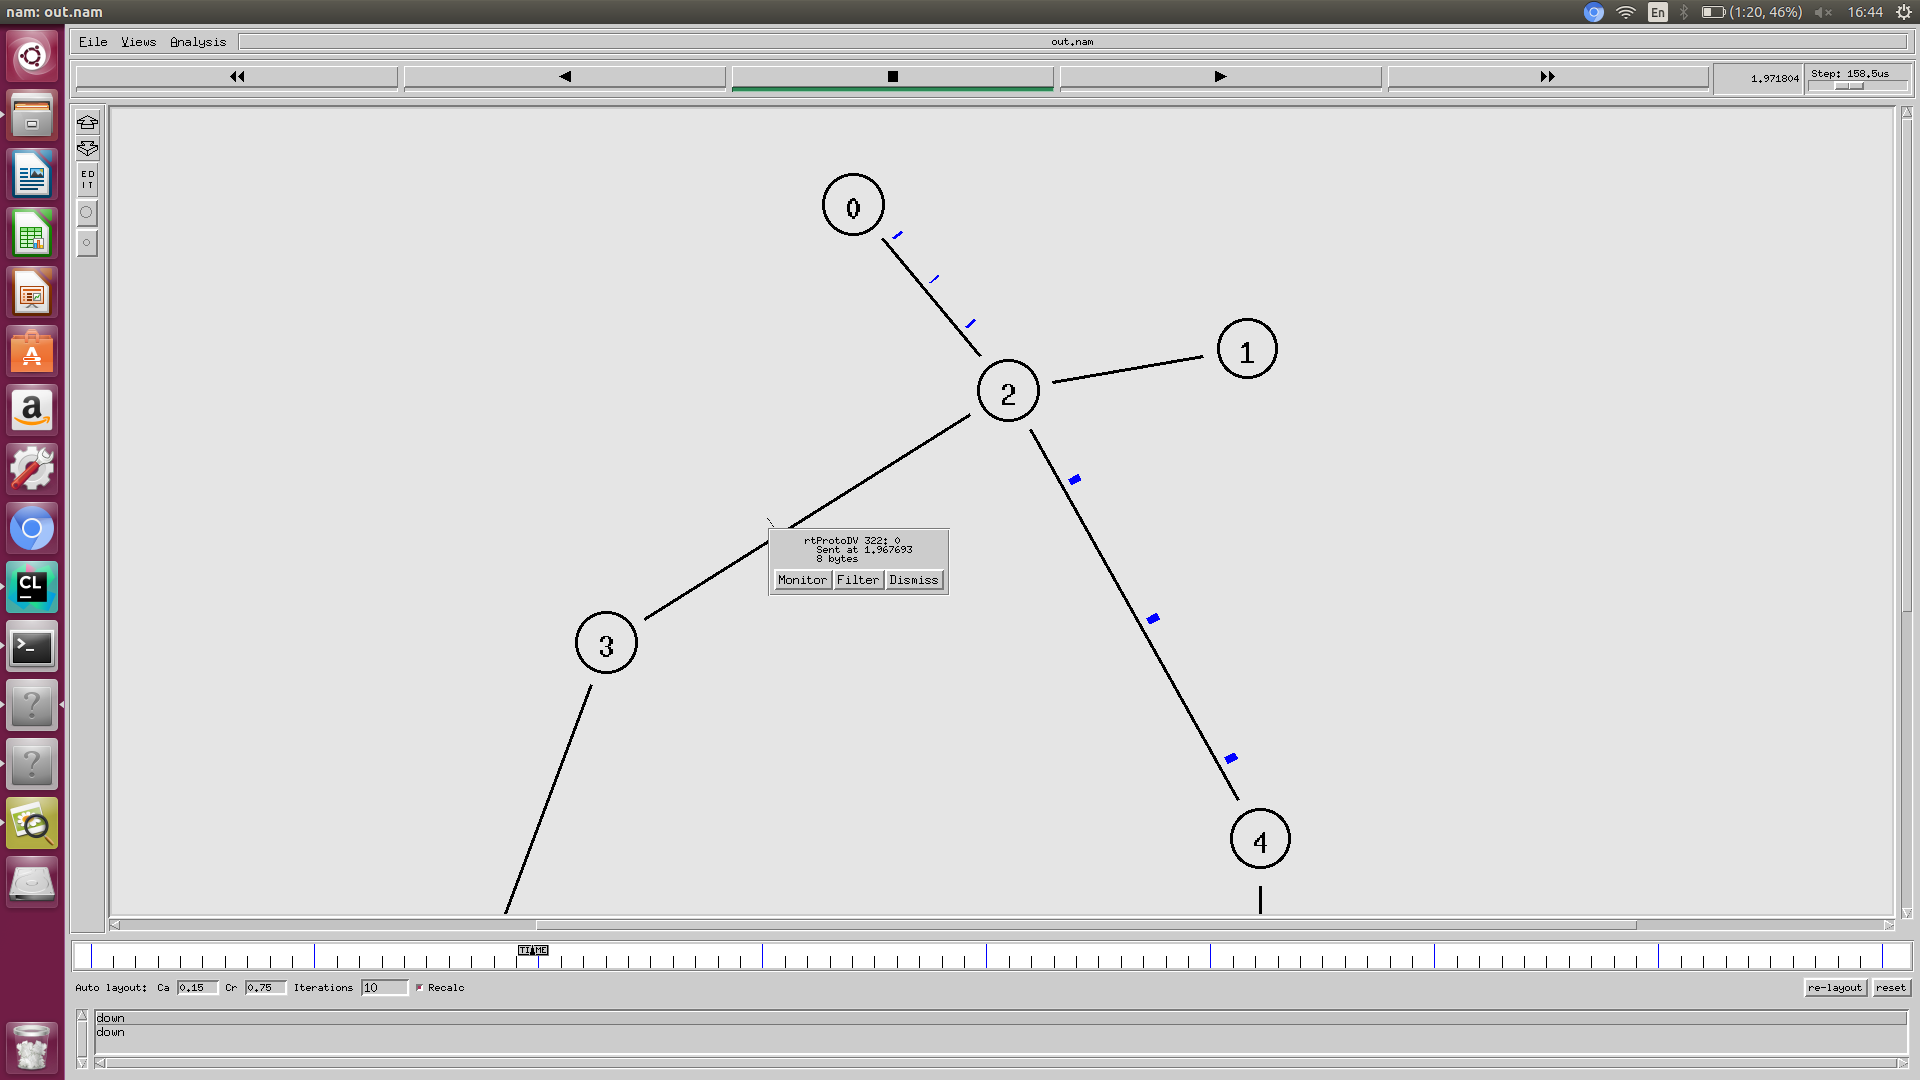
\includegraphics[width=0.99\columnwidth]{./tp2/tp2-1-DV-1-period.png}
    \caption{Paquets périodiques pour le routage}
    \end{figure}

    \begin{figure}
    \centering
    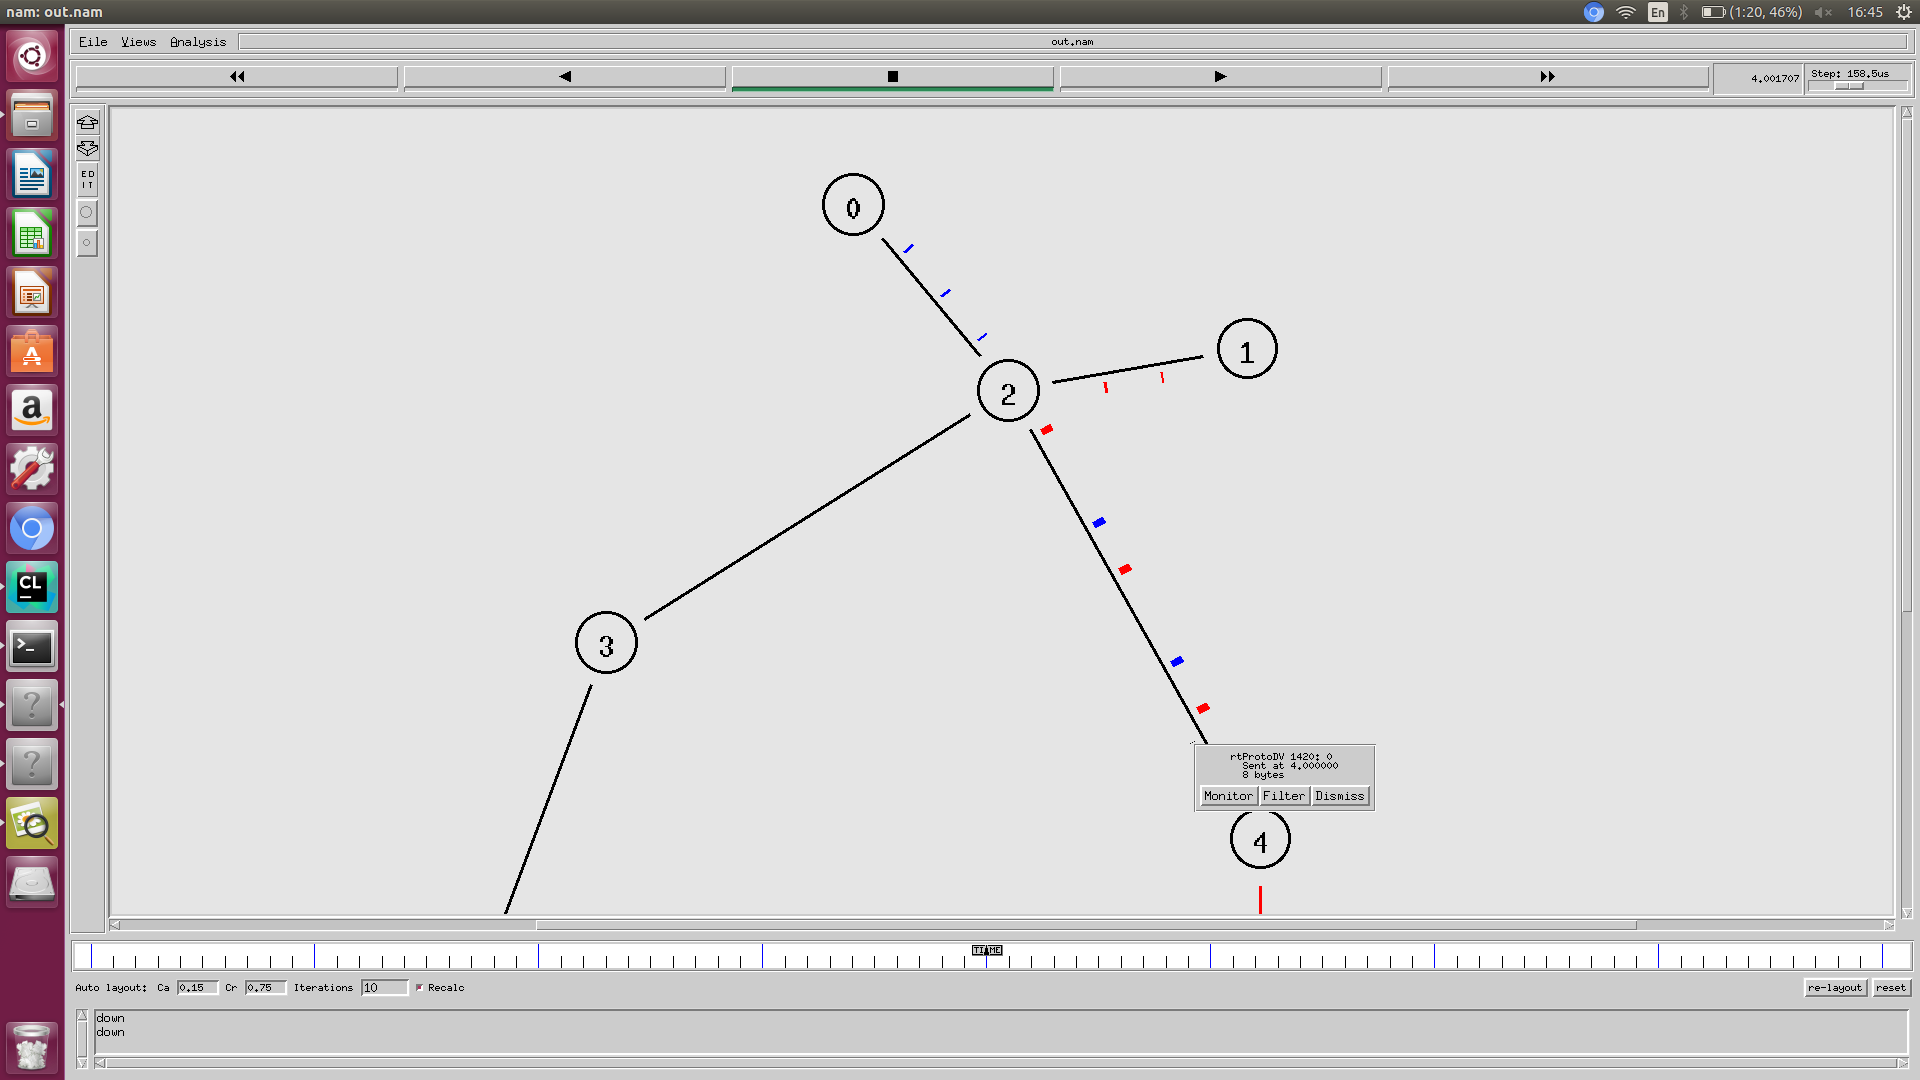
\includegraphics[width=0.99\columnwidth]{./tp2/tp2-1-DV-2-cut.png}
    \caption{Moment après la rupture}
    \end{figure}

    \begin{figure}
    \centering
    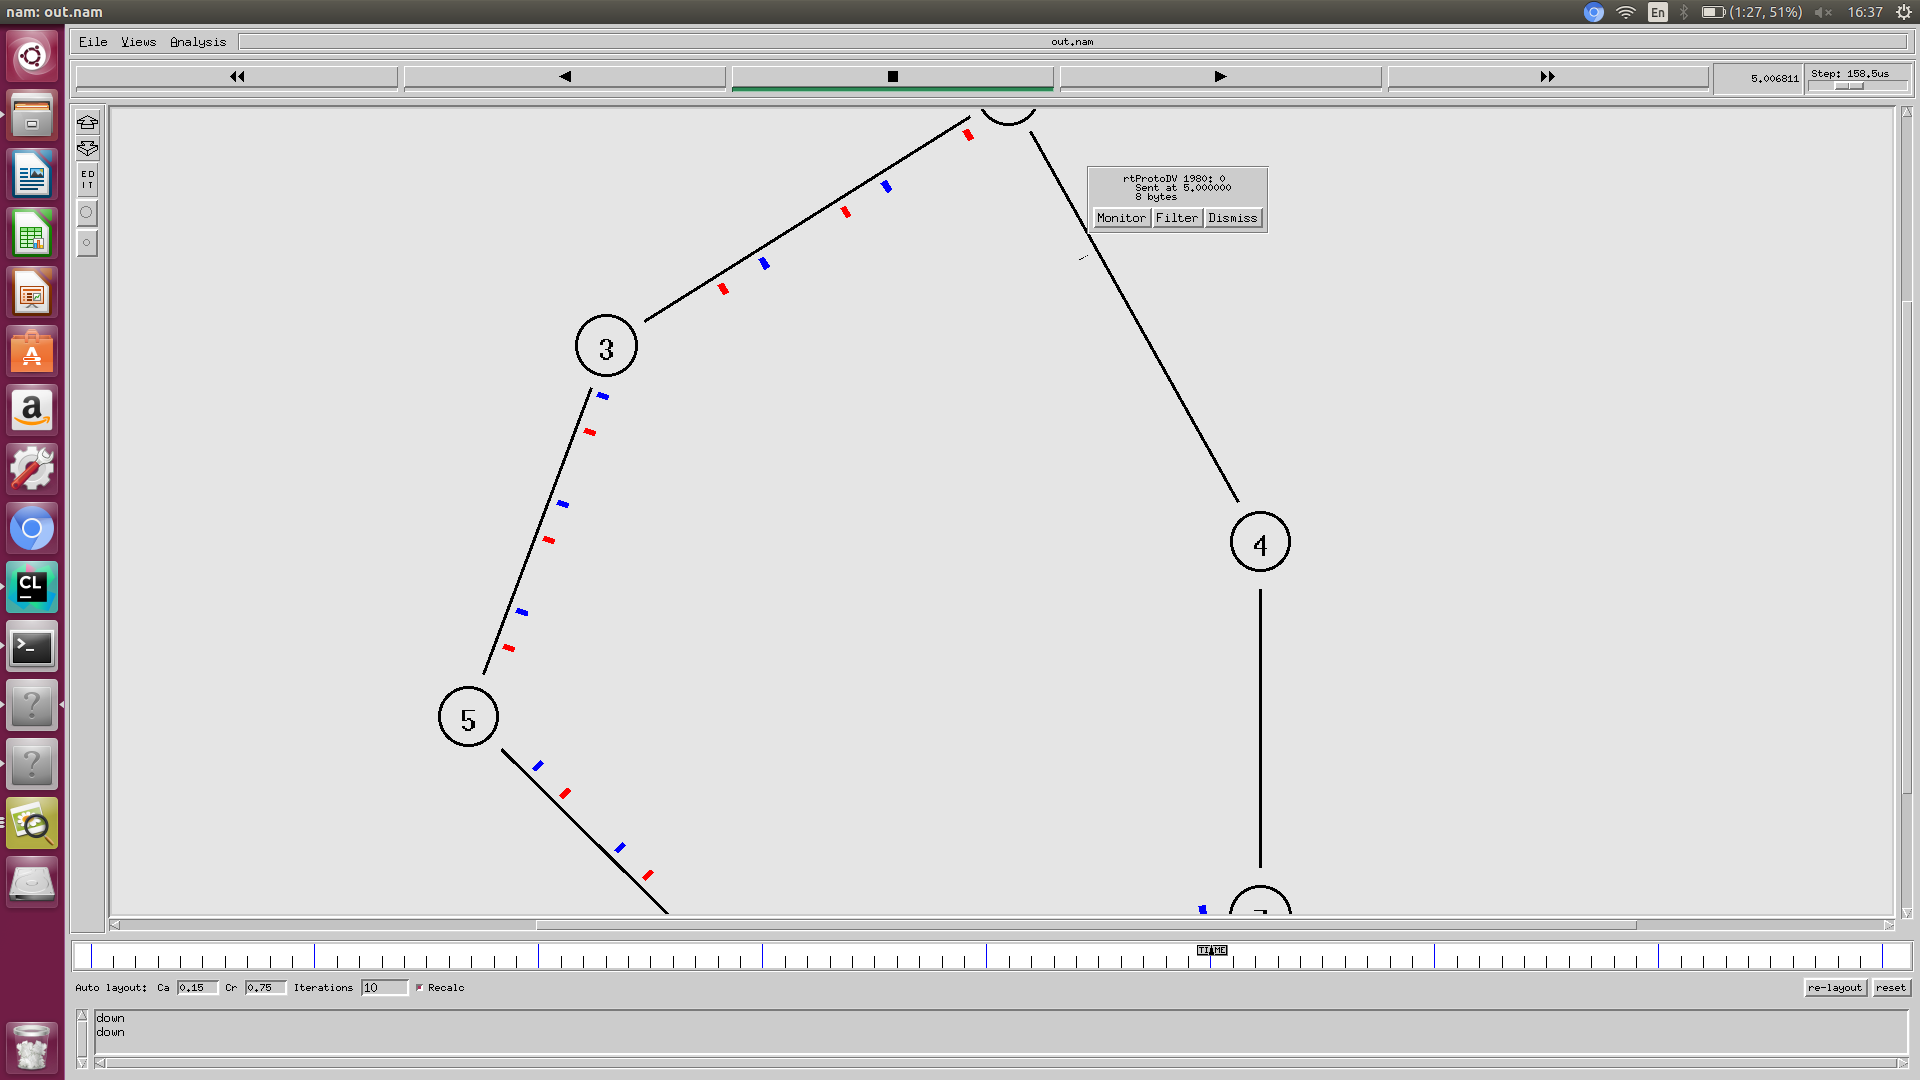
\includegraphics[width=0.99\columnwidth]{./tp2/tp2-1-DV-4-relink.png}
    \caption{Moment après le rétablissement de la jonction}
    \end{figure}

    \begin{figure}
    \centering
    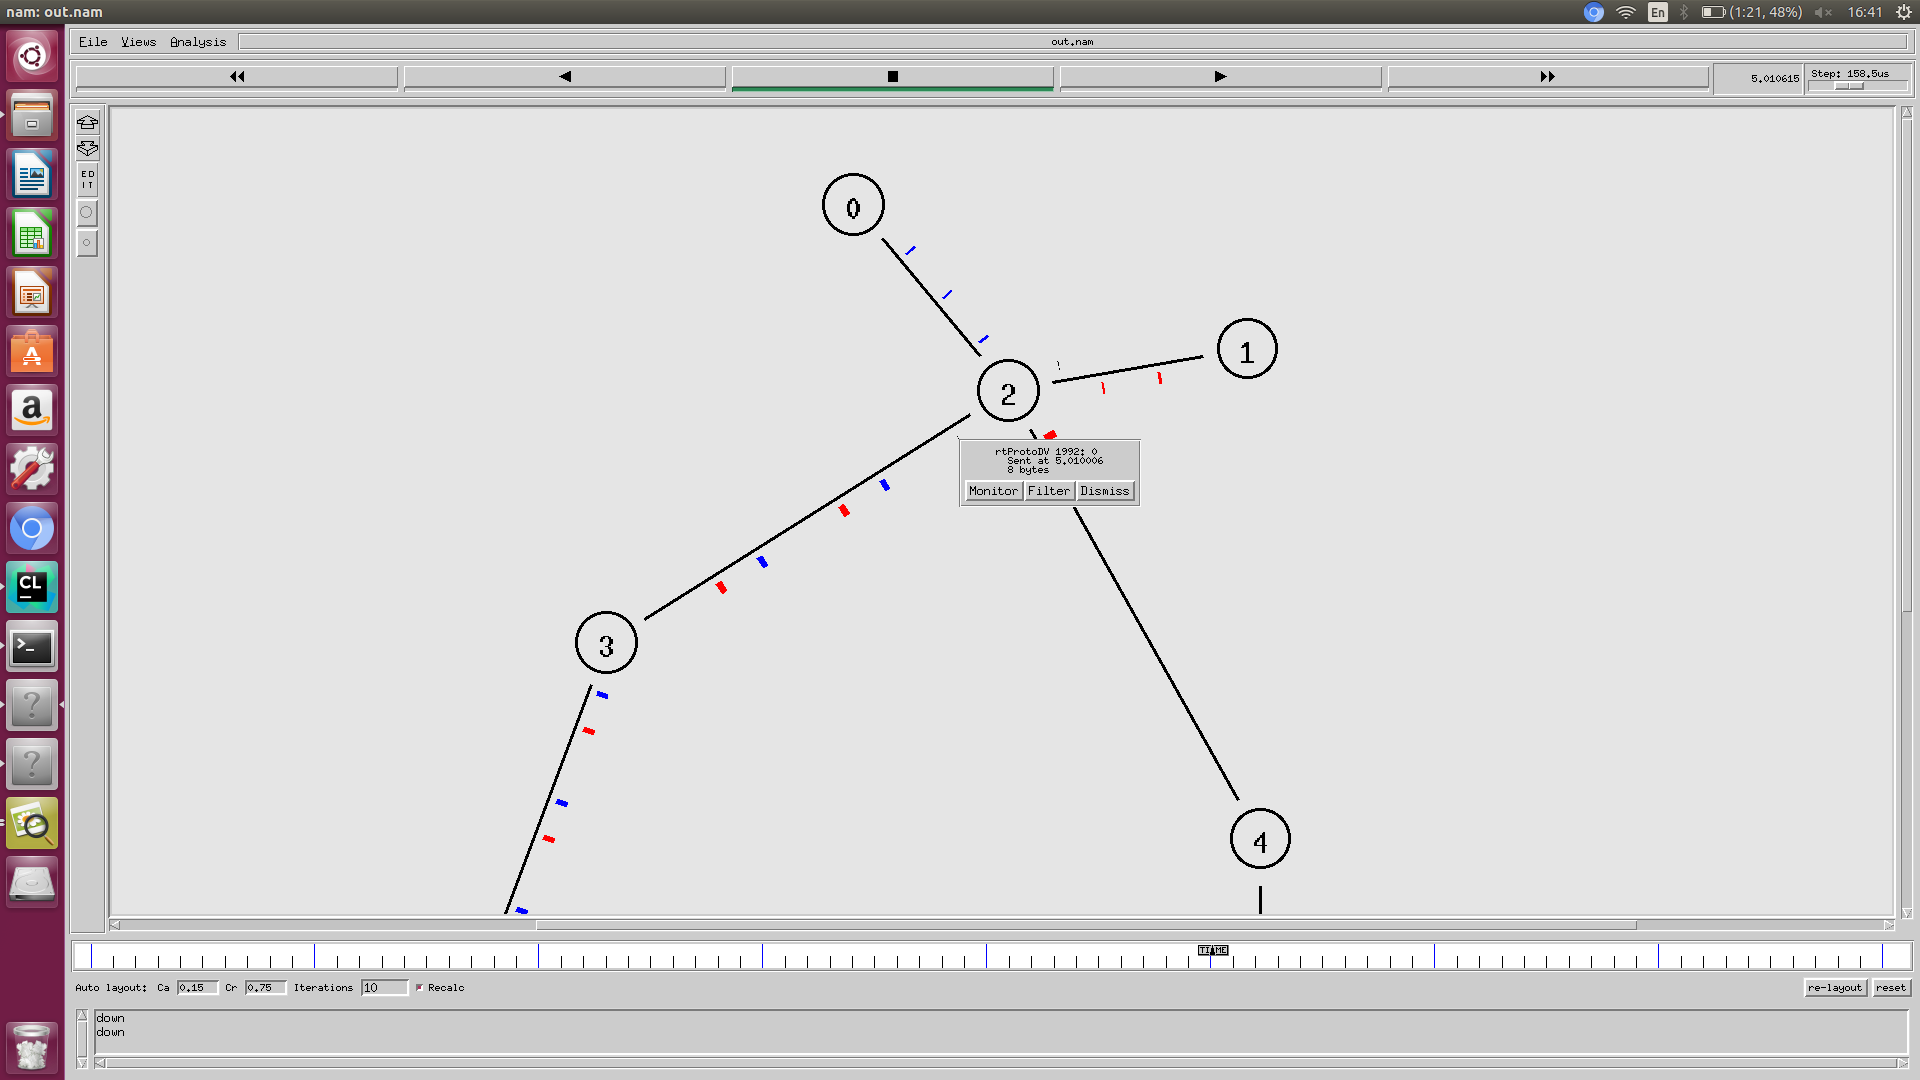
\includegraphics[width=0.99\columnwidth]{./tp2/tp2-1-DV-5-relink_triggered.png}
    \caption{Routage refait après le rétablissement de la jonction}
    \end{figure}

    \begin{figure}
    \centering
    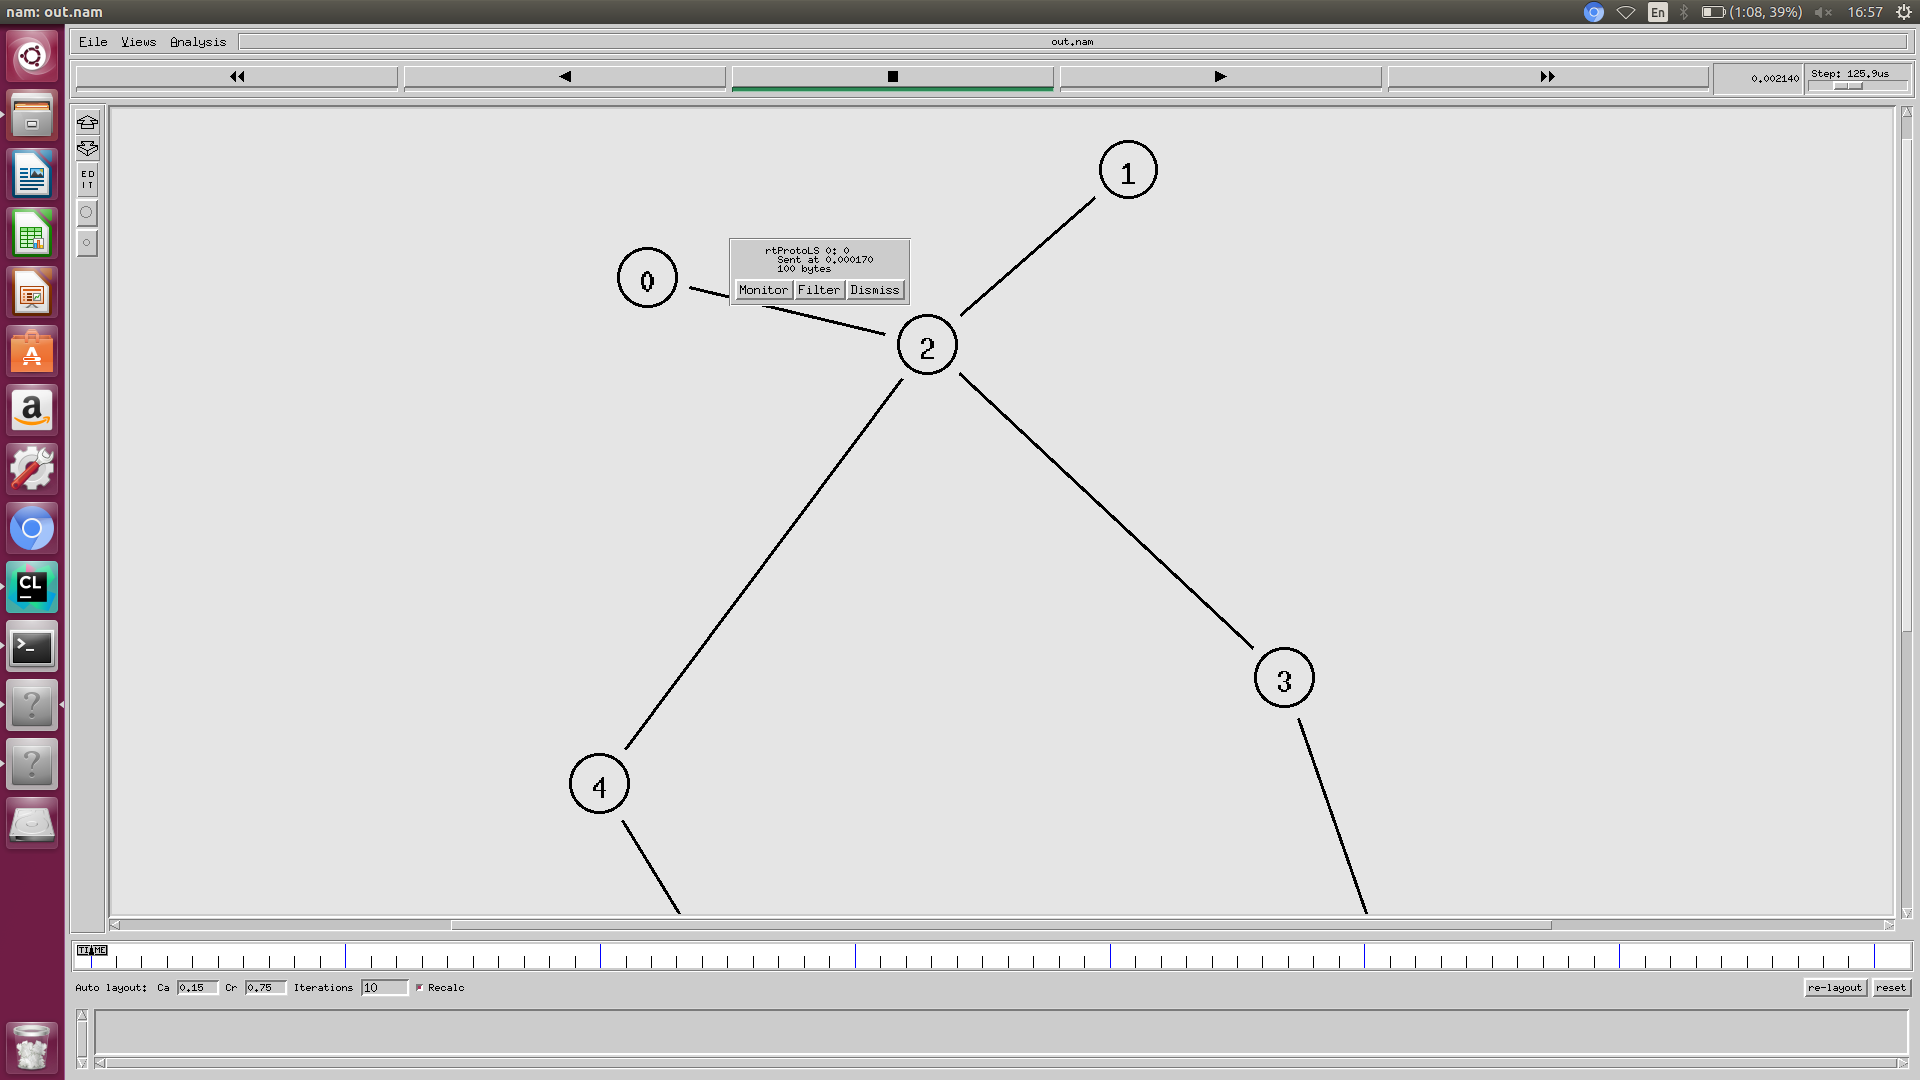
\includegraphics[width=0.99\columnwidth]{./tp2/tp2-1-LS-0-init.png}
    \caption{Paquets d'initialisation}
    \end{figure}
    \begin{figure}
    \centering
    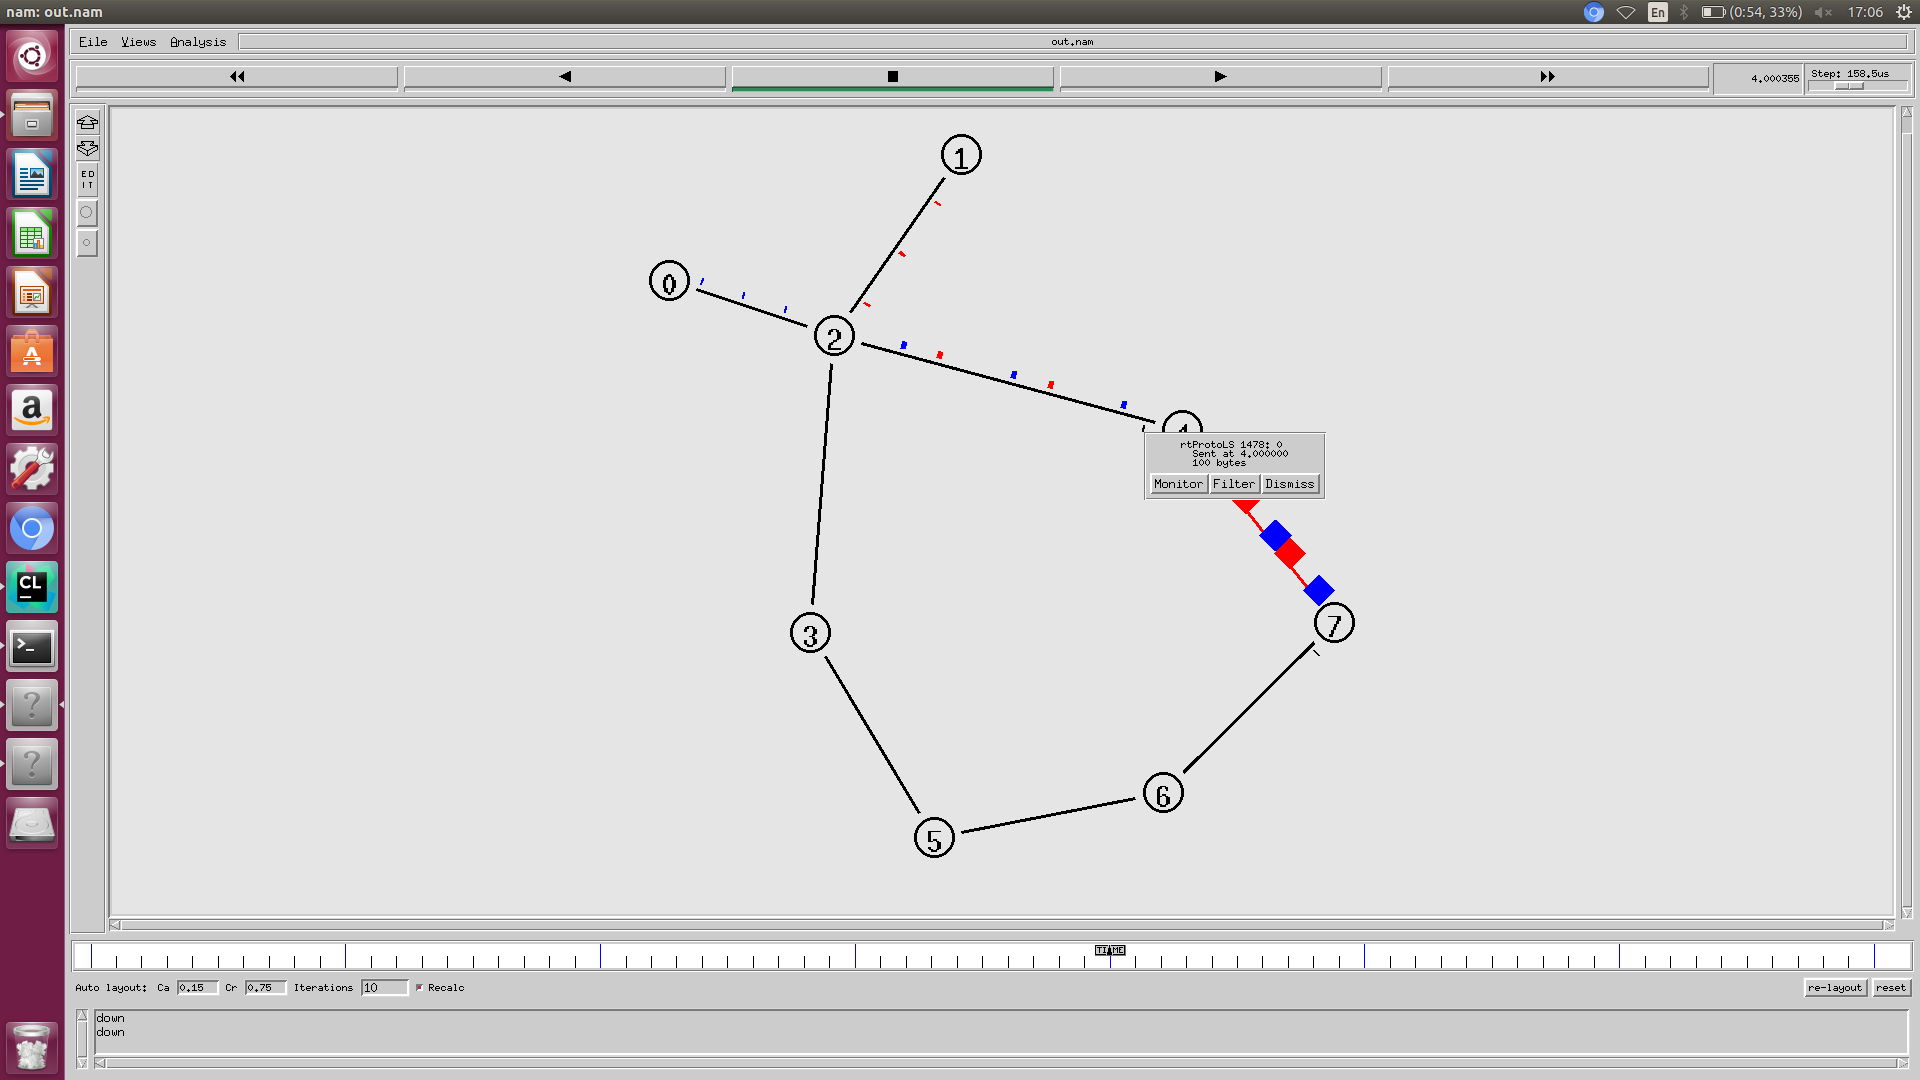
\includegraphics[width=0.99\columnwidth]{./tp2/tp2-1-LS-1-cut.png}
    \caption{Après la rupture de la jonction}
    \end{figure}
    \begin{figure}
    \centering
    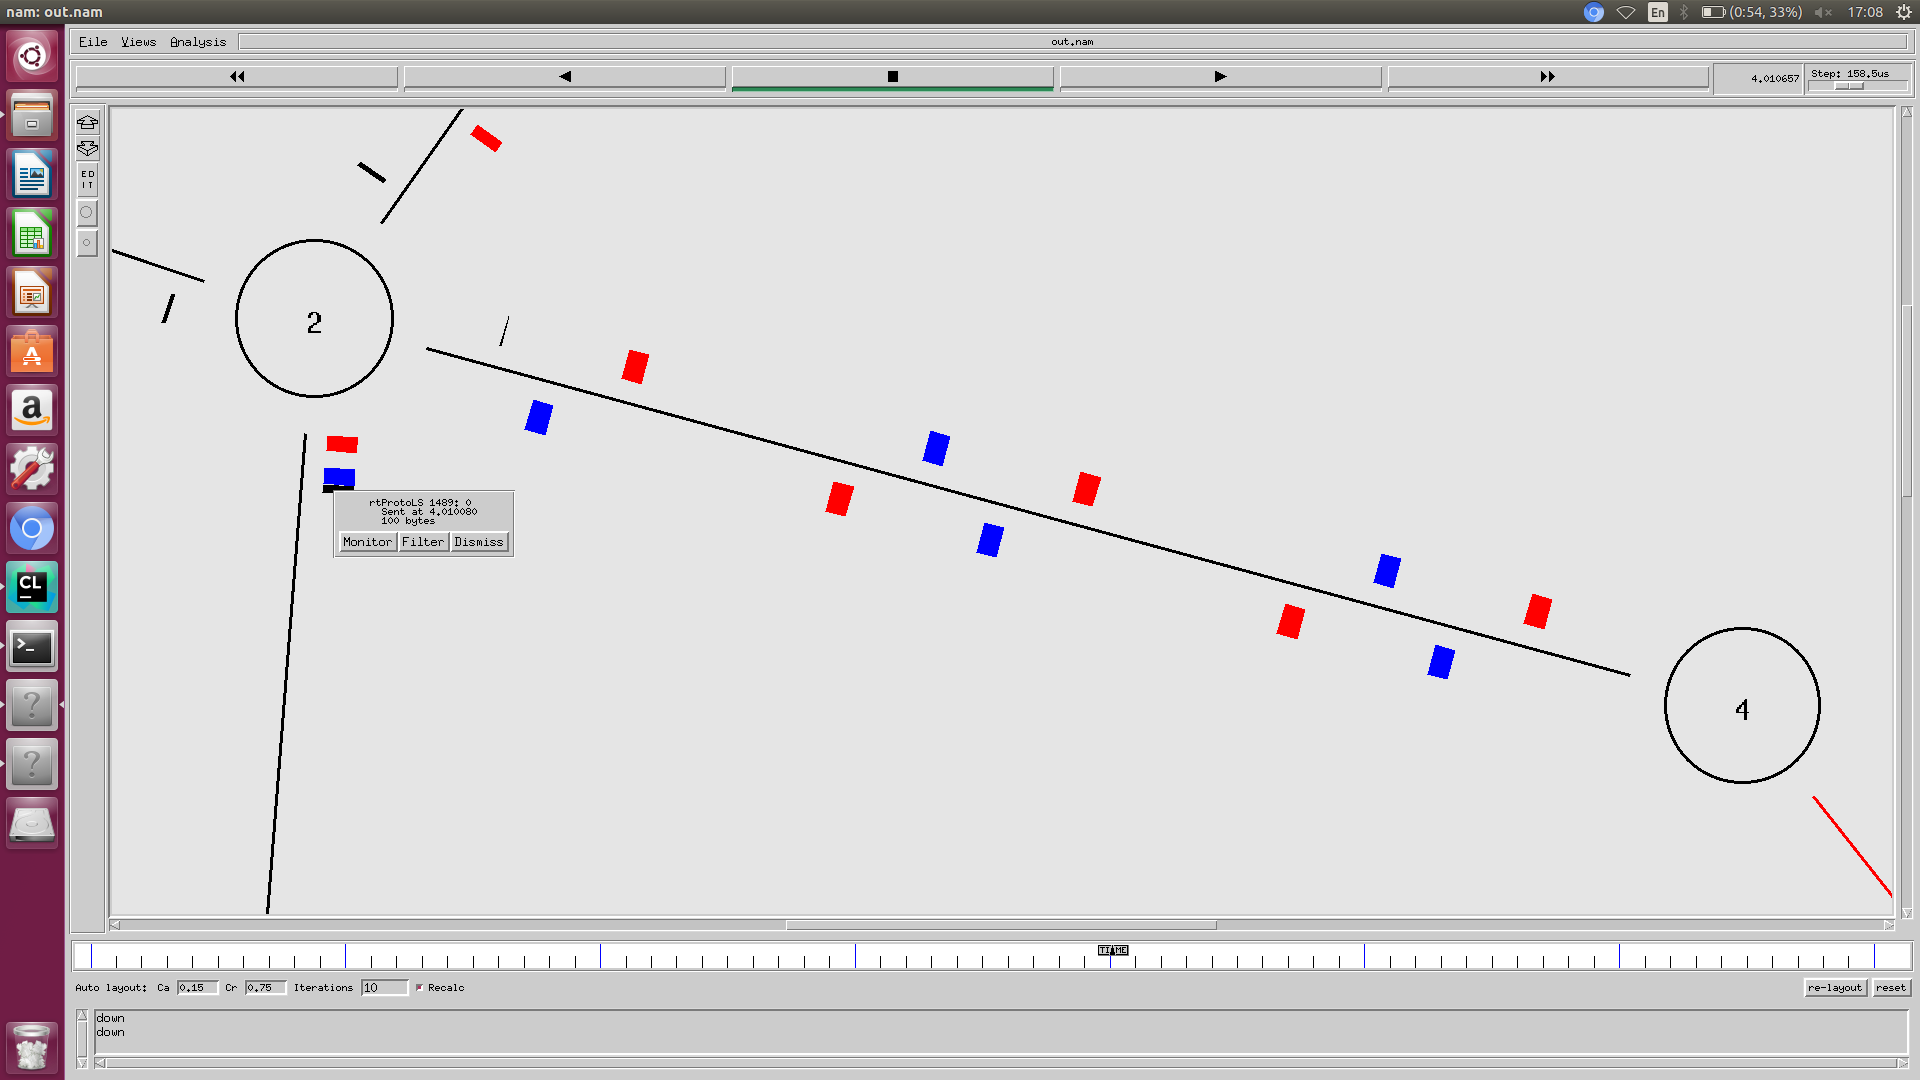
\includegraphics[width=0.99\columnwidth]{./tp2/tp2-1-LS-2-cut_riggered.png}
    \caption{Routage refait après la rupture}
    \end{figure}
    \begin{figure}
    \centering
    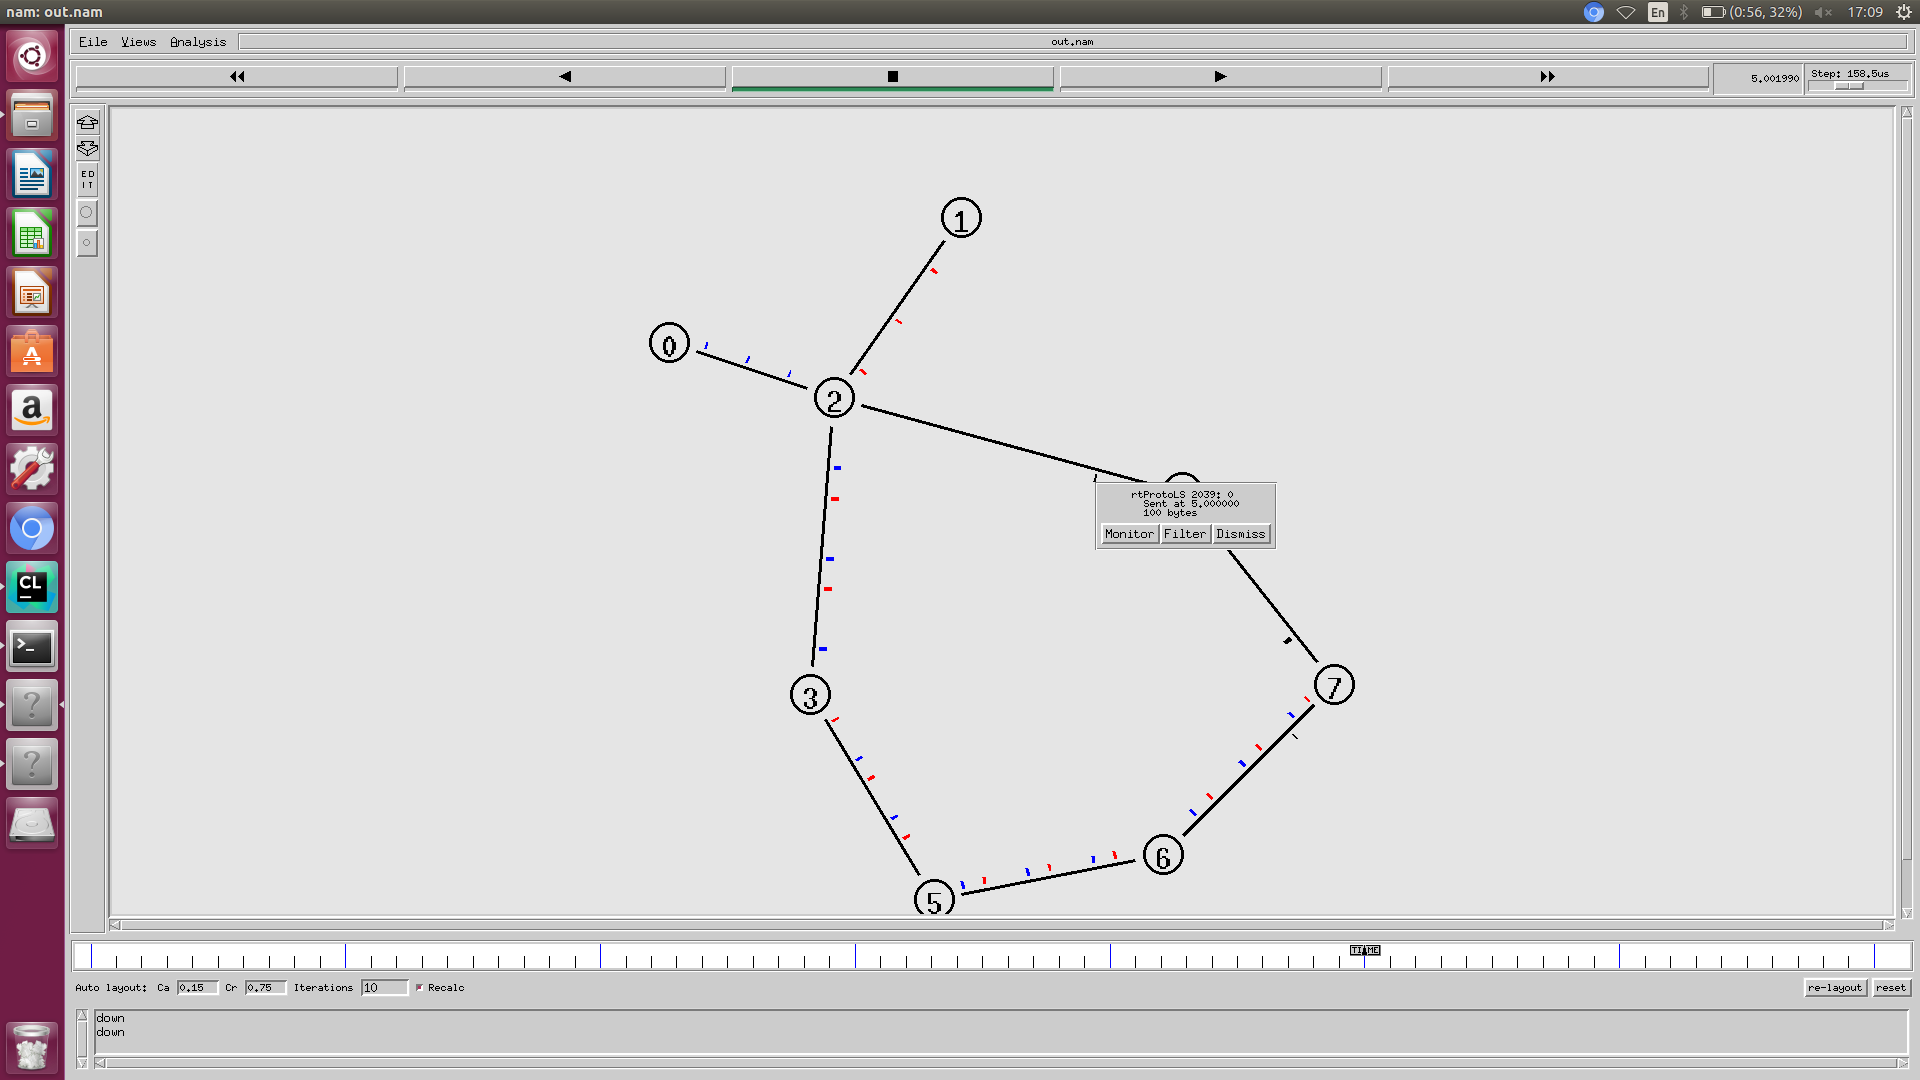
\includegraphics[width=0.99\columnwidth]{./tp2/tp2-1-LS-3-relink.png}
    \caption{Rétablissement de la jonction}
    \end{figure}
    \begin{figure}
    \centering
    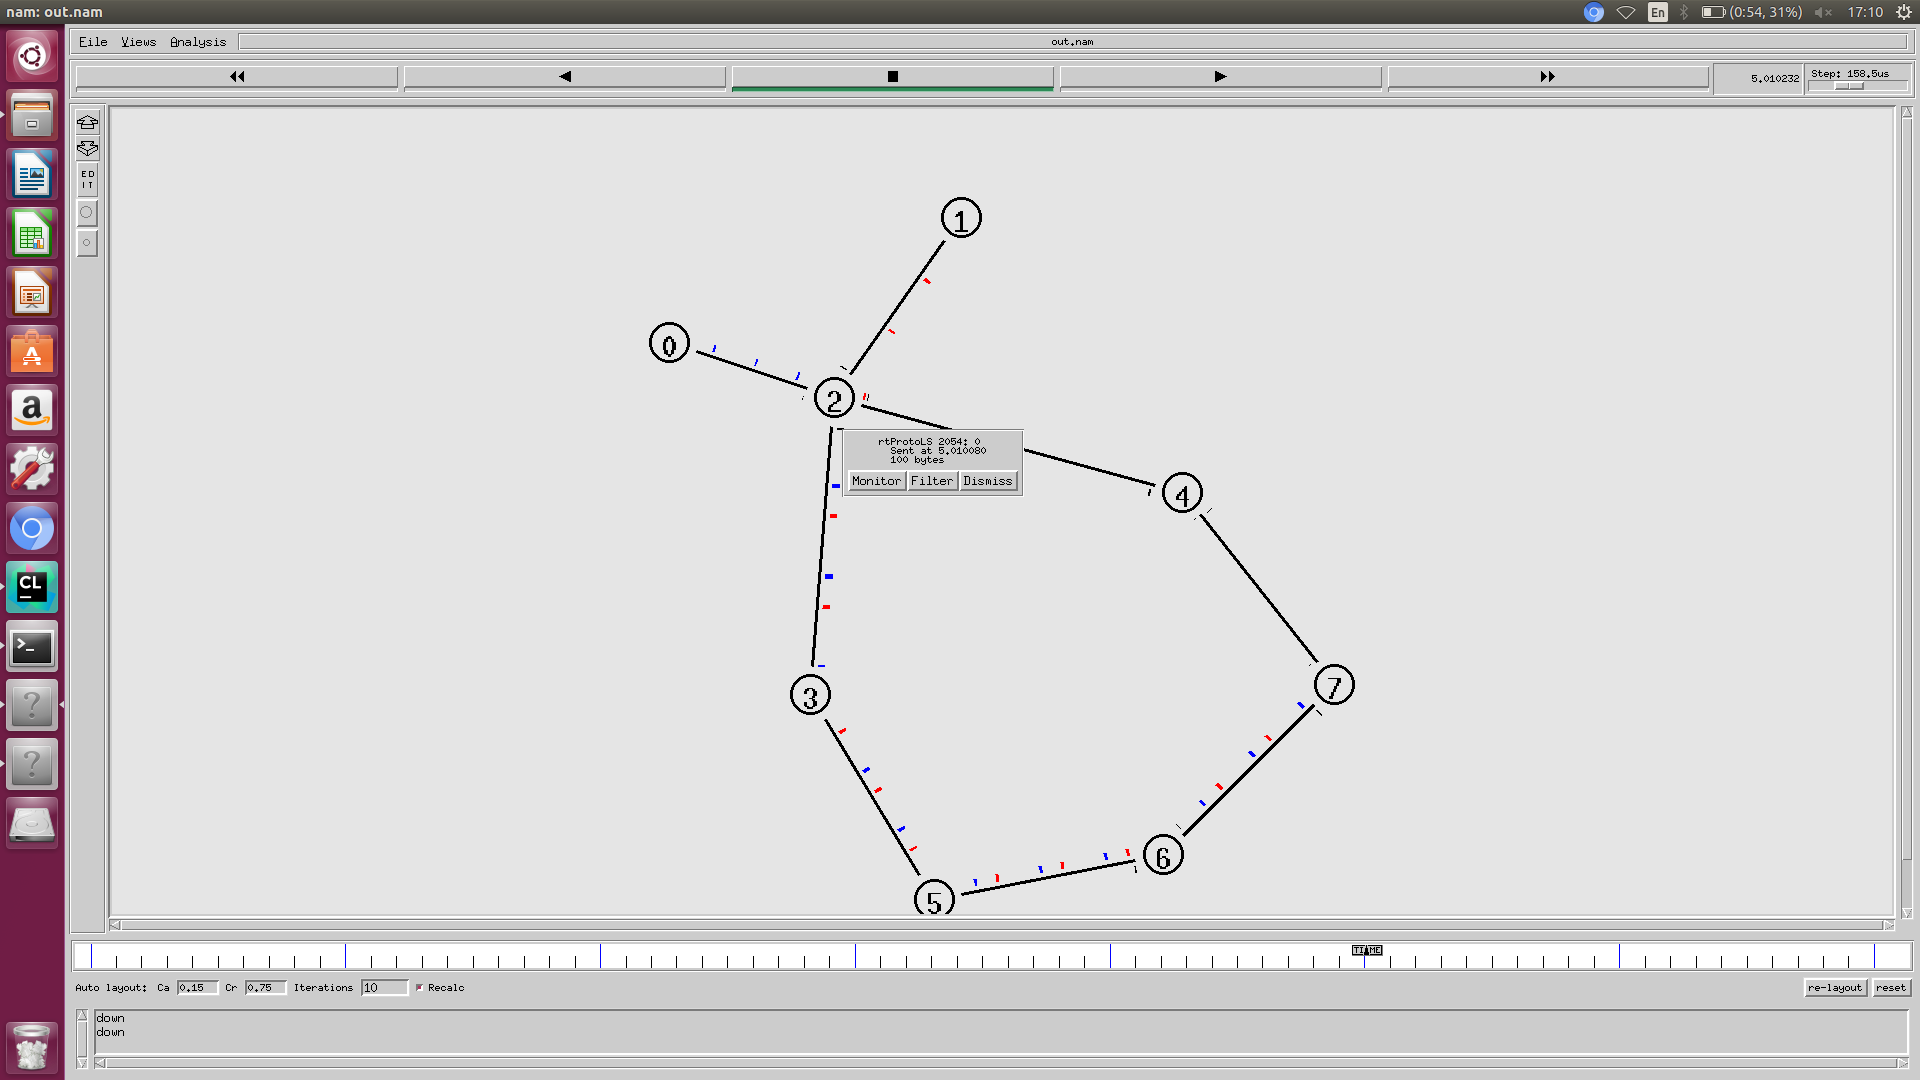
\includegraphics[width=0.99\columnwidth]{./tp2/tp2-1-LS-4-relink_triggered.png}
    \caption{Routage refait après le rétablissement de la jonction}
    \end{figure}
\end{document}
